% !TeX program = lualatex
\documentclass{article}
\usepackage[utf8]{inputenc}
\usepackage{amsmath}
\usepackage{tikz}
\usepackage{pgfplots, pgfplotstable}
\usetikzlibrary{calc}
\usepackage{pst-plot,pst-ode,multido}
\usepackage{derivative}

\pgfplotsset{ % Define a common style, so we don't repeat ourselves
	MyQuiver2D/.style={
		width=0.6\textwidth, % Overall width of the plot
		axis equal image, % Unit vectors for both axes have the same length
		view={0}{90}, % We need to use "3D" plots, but we set the view so we look at them from straight up
		xmin=-5.1, xmax=5.1, % Axis limits
		ymin=-5.1, ymax=5.1,
		domain=-5:5, y domain=-5:5, % Domain over which to evaluate the functions
		xtick={-5,-4,...,5}, ytick={-5,-4,...,5}, % Tick marks %
		samples=21, % How many arrows?
		cycle list={    % Plot styles
			gray,
			quiver={
				u={f(x,y)}, v={g(x,y)}, % End points of the arrows
				scale arrows=0.015,
				every arrow/.append style={
					-latex % Arrow tip
				},
			}\\
			red, samples=31, smooth, very thick, no markers, domain=-5:5 \\ % The plot style for the function
		}
	}
}

\definecolor[ps]{random}{rgb}{Rand Rand Rand}
\def\odeRHSone{
	x[0]*(x[0]-1)-x[1]+1
	|
	x[0]-x[1]
}
\def\odeRHStwo{
	x[0]^2/x[1] - x[0]
	|
	x[0]^2 - 2*x[1]
}
\def\odeRHSfouraone{
	x[0]*(x[0]-1)-x[1]+0.5
	|
	x[0]-x[1]
}
\def\odeRHSfouratwo{
	x[0]*(x[0]-1)-x[1]+1.5
	|
	x[0]-x[1]
}
\def\odeRHSfourathree{
	-1-x[0]^2
	|
	-x[1]
}
\def\odeRHSfourbone{
	x[1]-2*x[0]
	|
	2+x[0]^2-x[1]
}
\def\odeRHSfourbtwo{
	x[1]-2*x[0]
	|
	1+x[0]^2-x[1]
}
\def\odeRHSfourbthree{
	x[1]-2*x[0]
	|
	0+x[0]^2-x[1]
}
\def\odeRHSfourbfour{
	x[1]-2*x[0]
	|
	-17/64+x[0]^2-x[1]
}
\def\odeRHSfourbfive{
	x[1]-2*x[0]
	|
	-1+x[0]^2-x[1]
}
\def\odeRHSfiveaone{
	0*x[0]-x[0]^2
	|
	-x[1]
}
\def\odeRHSfiveatwo{
	1*x[0]-x[0]^2
	|
	-x[1]
}
\def\odeRHSfiveathree{
	-1*x[0]-x[0]^2
	|
	-x[1]
}
\def\odeRHSfivebone{
	x[1]-2*x[0]
	|
	-x[1]+x[0]/(x[0]+1)
}
\def\odeRHSfivebtwo{
	x[1]-1*x[0]
	|
	-x[1]+x[0]/(x[0]+1)
}
\def\odeRHSfivebthree{
	x[1]-0*x[0]
	|
	-x[1]+x[0]/(x[0]+1)
}
\def\odeRHSfivebfour{
	x[1]--1*x[0]
	|
	-x[1]+x[0]/(x[0]+1)
}
\def\odeRHSfivebfive{
	x[1]--2*x[0]
	|
	-x[1]+x[0]/(x[0]+1)
}

\title{HW 8}
\author{Ravi Kini}
\date{March 2023}

\begin{document}
	\maketitle
	\begin{enumerate}
		\item
		\begin{enumerate}
			\item [I.]
			\begin{enumerate}
				\item [a.]
				\begin{equation}
					\begin{split}
						\frac{dv}{dt} = 0 & = v(v - 1) - w + 1 \\
						w^* & = v^2 - v + 1 \\
						\frac{dw}{dt} = 0 & = v - w \\
						w^* & = v^* \\
						(v^*, w^*) & = (1,1) \\
						\operatorname{DF}(v,w) & = \begin{bmatrix} 2v - 1 & -1 \\ 1 & -1\end{bmatrix} \\
						(2v - 1 - \lambda)(-1-\lambda) + 1 & = 0 \\
						\lambda & = v - 1 \pm \sqrt{v^2 - 1} \\
						\lambda_{(1,1)} & = 0
					\end{split}
				\end{equation}
				
				No conclusions can be made using linear stability analysis about the stability of the steady state $(1,1)$.
				\item [b.]
				The v-nullclines are in blue, and the w-nullclines in red.
		
		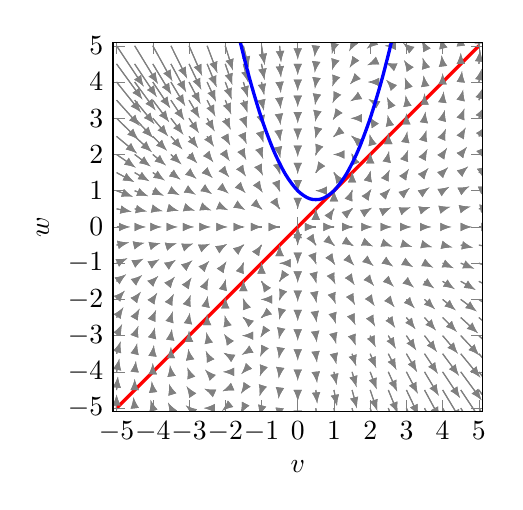
\begin{tikzpicture}[
			declare function={f(\x,\y) = \x*(\x-\y);},
			declare function={g(\x,\y) = \y*(2*\x-\y);}
			]
			\begin{axis}[
				MyQuiver2D,
				xlabel={$v$},ylabel={$w$}]
				\addplot3 (x,y,0);
				\addplot +[red] ({x},{x});
				\addplot3 (x,y,0);
				\addplot +[blue] ({x},{x^2 - x + 1});
			\end{axis}
		\end{tikzpicture}
		
		\psset{unit=0.5}
		\begin{pspicture}(-5.2,-5.2)(5.1,5.1)
			\psaxes[ticksize=0 4pt,axesstyle=frame,tickstyle=inner,
			Ox=-5,Oy=-5](-5,-5)(5,5)
			\psset{arrows=->,algebraic}
			\rput(-0.5,-6.5){$v$}
			\rput(-6.5,-0.5){$w$}
			\pstODEsolve[algebraicAll]{sol_1_1}{x[0] | x[1]}{0}{0.5}{100}{2 | 2}{\odeRHSone}
			\pstODEsolve[algebraicAll]{sol_1_2}{x[0] | x[1]}{0}{2}{100}{2 | 4}{\odeRHSone}
			\pstODEsolve[algebraicAll]{sol_2_1}{x[0] | x[1]}{0}{0.2}{100}{4 | 2}{\odeRHSone}
			\pstODEsolve[algebraicAll]{sol_n1_n1}{x[0] | x[1]}{0}{2}{100}{-2 | -2}{\odeRHSone}
			\pstODEsolve[algebraicAll]{sol_n1_n2}{x[0] | x[1]}{0}{0.2}{100}{-2 | -4}{\odeRHSone}
			\pstODEsolve[algebraicAll]{sol_n2_n1}{x[0] | x[1]}{0}{0.5}{100}{-4 | -2}{\odeRHSone}
			\pstODEsolve[algebraicAll]{sol_1_n1}{x[0] | x[1]}{0}{0.2}{100}{2 | -2}{\odeRHSone}
			\pstODEsolve[algebraicAll]{sol_n1_1}{x[0] | x[1]}{0}{5}{100}{-2 | 2}{\odeRHSone}
			
			
			\psset{arrows=->,linewidth=1pt}%
			\listplot[linecolor=random  ]{sol_1_1}
			\listplot[linecolor=random  ]{sol_1_2}
			\listplot[linecolor=random  ]{sol_2_1}
			\listplot[linecolor=random  ]{sol_n1_n1}
			\listplot[linecolor=random  ]{sol_n1_n2}
			\listplot[linecolor=random  ]{sol_n2_n1}
			\listplot[linecolor=random  ]{sol_1_n1}
			\listplot[linecolor=random  ]{sol_n1_1}
		\end{pspicture}
		\\
		\\
		\\
				\item [c.] This fixed point behaves like a mixture of a saddle point and a spiral, so an appropriate term could be "saddle spiral".
			\end{enumerate}
			\item [II.]
			\begin{enumerate}
				\item [a.]
				\begin{equation}
					\begin{split}
						\frac{dv}{dt} = 0 & = v(v - 1) - w + I \\
						w^* & = v^2 - v + I \\
						\frac{dw}{dt} = 0 & = v - w \\
						w^* & = v^* \\
						(v^*, w^*) & = (1\pm\sqrt{1-I},1\pm\sqrt{1-I}) \\
						\operatorname{DF}(v,w) & = \begin{bmatrix} 2v - 1 & -1 \\ 1 & -1\end{bmatrix} \\
						(2v - 1 - \lambda)(-1-\lambda) + 1 & = 0 \\
						\lambda & = v - 1 \pm \sqrt{v^2 - 1} \\
						\lambda_{(1+\sqrt{1-I},1+\sqrt{1-I})} & = \sqrt{1-x} \pm \sqrt{1-x+2\sqrt{1-x}} \\
						\lambda_{(1-\sqrt{1-I},1-\sqrt{1-I})} & = -\sqrt{1-x} \pm \sqrt{1-x-2\sqrt{1-x}}
					\end{split}
				\end{equation}
				
				If $-\infty < I < -3$, there is a saddle point at $(1+\sqrt{1-I},1+\sqrt{1-I})$ and a stable node at $(1-\sqrt{1-I},1-\sqrt{1-I})$.
				
				If $-3 \leq I \leq 1$, there is a saddle point at $(1+\sqrt{1-I},1+\sqrt{1-I})$ and a stable spiral at $(1-\sqrt{1-I},1-\sqrt{1-I})$.
				
				If $I = 1$, there is a saddle spiral at $(1-\sqrt{1-I},1-\sqrt{1-I})$.
				
				If $1 < I < \infty$, there are no steady states.
				\item [b.]
				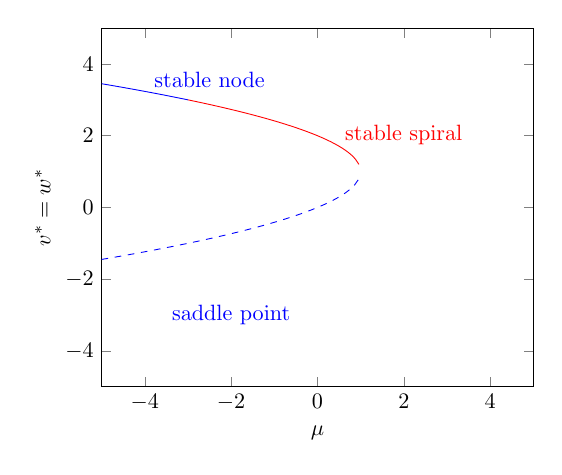
\begin{tikzpicture}[scale=0.8]
					\begin{axis}[xmin=-5,xmax=5,ymin=-5,ymax=5,
						restrict x to domain=-5:5,restrict y to domain=-5:5,xlabel={$\mu$},ylabel={$v^*=w^*$}]
						\addplot[color=blue,dashed,samples=100,domain=-5:5]{1-sqrt(1-x)};	\addplot[color=blue,solid,samples=100,domain=-5:-3]{1+sqrt(1-x)};\addplot[color=red,solid,samples=100,domain=-3:5]{1+sqrt(1-x)};
						\node[blue,below,align=center] at (axis cs:-2.5,4){stable node};
						\node[red,below,align=center] at (axis cs:2,2.5){stable spiral};
						\node[blue,below,align=center] at (axis cs:-2,-2.5){saddle point};
					\end{axis}
				\end{tikzpicture}
			
			A saddle-node bifurcation occurs at $I = 1$.
				\item [c.]
				For $I = 0.5$, without loss of generality:
				
				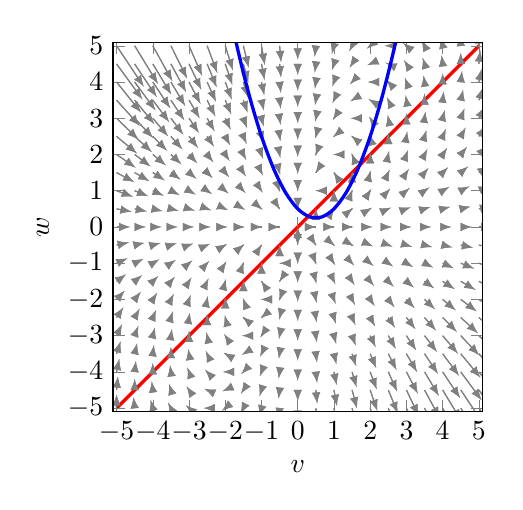
\begin{tikzpicture}[
			declare function={f(\x,\y) = \x*(\x-\y);},
			declare function={g(\x,\y) = \y*(2*\x-\y);}
			]
			\begin{axis}[
				MyQuiver2D,
				xlabel={$v$},ylabel={$w$}]
				\addplot3 (x,y,0);
				\addplot +[red] ({x},{x});
				\addplot3 (x,y,0);
				\addplot +[blue] ({x},{x^2 - x + 0.5});
			\end{axis}
		\end{tikzpicture}
		
		\psset{unit=0.5}
		\begin{pspicture}(-5.2,-5.2)(5.1,5.1)
			\psaxes[ticksize=0 4pt,axesstyle=frame,tickstyle=inner,
			Ox=-5,Oy=-5](-5,-5)(5,5)
			\psset{arrows=->,algebraic}
			\rput(-0.5,-6.5){$v$}
			\rput(-6.5,-0.5){$w$}
			\pstODEsolve[algebraicAll]{sol_1_1}{x[0] | x[1]}{0}{0.5}{100}{2 | 2}{\odeRHSfouraone}
			\pstODEsolve[algebraicAll]{sol_1_2}{x[0] | x[1]}{0}{2}{100}{2 | 4}{\odeRHSfouraone}
			\pstODEsolve[algebraicAll]{sol_2_1}{x[0] | x[1]}{0}{0.2}{100}{4 | 2}{\odeRHSfouraone}
			\pstODEsolve[algebraicAll]{sol_n1_n1}{x[0] | x[1]}{0}{2}{100}{-2 | -2}{\odeRHSfouraone}
			\pstODEsolve[algebraicAll]{sol_n1_n2}{x[0] | x[1]}{0}{0.2}{100}{-2 | -4}{\odeRHSfouraone}
			\pstODEsolve[algebraicAll]{sol_n2_n1}{x[0] | x[1]}{0}{0.5}{100}{-4 | -2}{\odeRHSfouraone}
			\pstODEsolve[algebraicAll]{sol_1_n1}{x[0] | x[1]}{0}{0.2}{100}{2 | -2}{\odeRHSfouraone}
			\pstODEsolve[algebraicAll]{sol_n1_1}{x[0] | x[1]}{0}{5}{100}{-2 | 2}{\odeRHSfouraone}
			
			
			\psset{arrows=->,linewidth=1pt}%
			\listplot[linecolor=random  ]{sol_1_1}
			\listplot[linecolor=random  ]{sol_1_2}
			\listplot[linecolor=random  ]{sol_2_1}
			\listplot[linecolor=random  ]{sol_n1_n1}
			\listplot[linecolor=random  ]{sol_n1_n2}
			\listplot[linecolor=random  ]{sol_n2_n1}
			\listplot[linecolor=random  ]{sol_1_n1}
			\listplot[linecolor=random  ]{sol_n1_1}
		\end{pspicture}
		\\
		\\
		\\
		For $I = 1.5$, without loss of generality:
		
				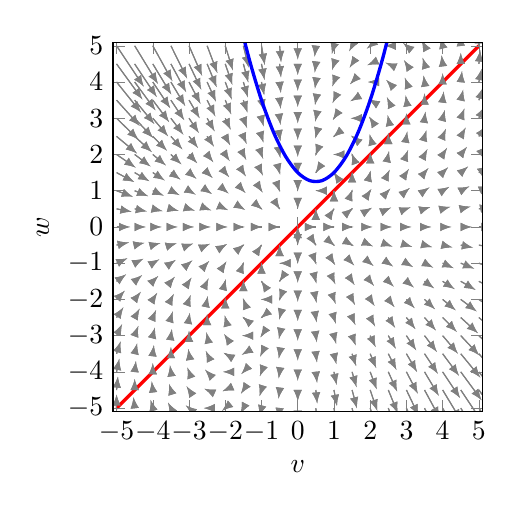
\begin{tikzpicture}[
			declare function={f(\x,\y) = \x*(\x-\y);},
			declare function={g(\x,\y) = \y*(2*\x-\y);}
			]
			\begin{axis}[
				MyQuiver2D,
				xlabel={$v$},ylabel={$w$}]
				\addplot3 (x,y,0);
				\addplot +[red] ({x},{x});
				\addplot3 (x,y,0);
				\addplot +[blue] ({x},{x^2 - x + 1.5});
			\end{axis}
		\end{tikzpicture}
		
		\psset{unit=1}
		\begin{pspicture}(-5.2,-5.2)(5.1,5.1)
			\psaxes[ticksize=0 4pt,axesstyle=frame,tickstyle=inner,
			Ox=-5,Oy=-5](-5,-5)(5,5)
			\psset{arrows=->,algebraic}
			\rput(-0.5,-6.5){$v$}
			\rput(-6.5,-0.5){$w$}
			\pstODEsolve[algebraicAll]{sol_1_1}{x[0] | x[1]}{0}{0.5}{100}{2 | 2}{\odeRHSfouratwo}
			\pstODEsolve[algebraicAll]{sol_1_2}{x[0] | x[1]}{0}{0.2}{100}{2 | 4}{\odeRHSfouratwo}
			\pstODEsolve[algebraicAll]{sol_2_1}{x[0] | x[1]}{0}{0.2}{100}{4 | 2}{\odeRHSfouratwo}
			\pstODEsolve[algebraicAll]{sol_n1_n1}{x[0] | x[1]}{0}{0.2}{100}{-2 | -2}{\odeRHSfouratwo}
			\pstODEsolve[algebraicAll]{sol_n1_n2}{x[0] | x[1]}{0}{0.2}{100}{-2 | -4}{\odeRHSfouratwo}
			\pstODEsolve[algebraicAll]{sol_n2_n1}{x[0] | x[1]}{0}{0.5}{100}{-4 | -2}{\odeRHSfouratwo}
			\pstODEsolve[algebraicAll]{sol_1_n1}{x[0] | x[1]}{0}{0.2}{100}{2 | -2}{\odeRHSfouratwo}
			\pstODEsolve[algebraicAll]{sol_n1_1}{x[0] | x[1]}{0}{0.5}{100}{-2 | 2}{\odeRHSfouratwo}
			
			
			\psset{arrows=->,linewidth=1pt}%
			\listplot[linecolor=random  ]{sol_1_1}
			\listplot[linecolor=random  ]{sol_1_2}
			\listplot[linecolor=random  ]{sol_2_1}
			\listplot[linecolor=random  ]{sol_n1_n1}
			\listplot[linecolor=random  ]{sol_n1_n2}
			\listplot[linecolor=random  ]{sol_n2_n1}
			\listplot[linecolor=random  ]{sol_1_n1}
			\listplot[linecolor=random  ]{sol_n1_1}
		\end{pspicture}
			\end{enumerate}
		\end{enumerate}
		\item
		\begin{enumerate}
			\item [I.]
			The r-nullclines are in blue, and the $\theta$-nullclines in red.
			
			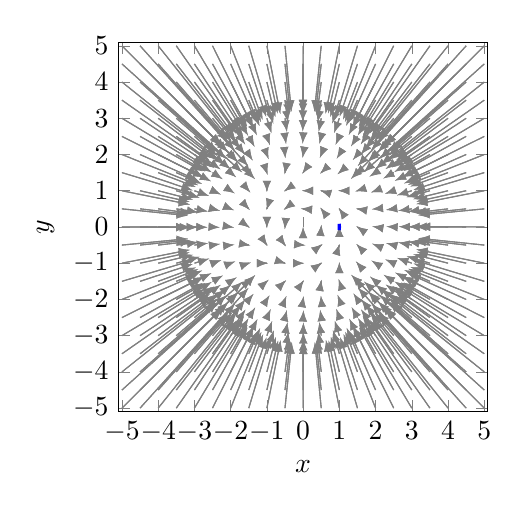
\begin{tikzpicture}[
			declare function={f(\x,\y) = (\x)/(sqrt(\x^2+\y^2))*sqrt(\x^2+\y^2)*(1-\x^2-\y^2)-(\y)/(sqrt(\x^2+\y^2))/sqrt(\x^2+\y^2)*2;},
			declare function={g(\x,\y) = (\y)/(sqrt(\x^2+\y^2))*sqrt(\x^2+\y^2)*(1-\x^2-\y^2)+(\x)/(sqrt(\x^2+\y^2))/sqrt(\x^2+\y^2)*2;}
			]
			\begin{axis}[
				MyQuiver2D,
				xlabel={$x$},ylabel={$y$}]
				\addplot3 (x,y,0);
				\addplot +[blue] ({0*cos(x)},{0*sin(x)});
				\addplot3 (x,y,0);
				\addplot +[blue] ({cos(x)},{sin(x)});
			\end{axis}
		\end{tikzpicture}
			\item [II.]
			The r-nullclines are in blue, and the $\theta$-nullclines in red.
			
			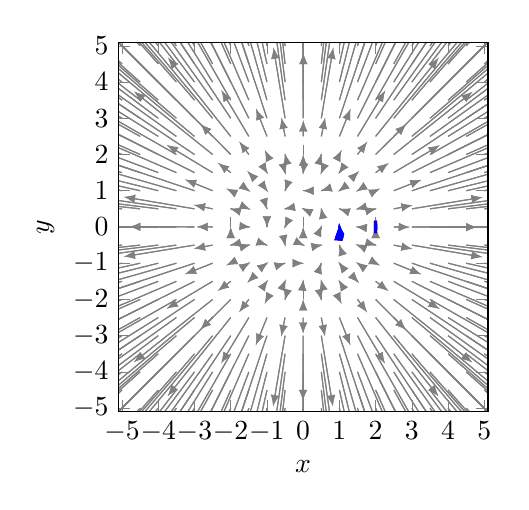
\begin{tikzpicture}[
			declare function={f(\x,\y) = (\x)/(sqrt(\x^2+\y^2))*sqrt(\x^2+\y^2)*(1-\x^2-\y^2)*(4-\x^2-\y^2)-(\y)/(sqrt(\x^2+\y^2))/sqrt(\x^2+\y^2)*(2-sqrt(\x^2+\y^2));},
			declare function={g(\x,\y) = (\y)/(sqrt(\x^2+\y^2))*sqrt(\x^2+\y^2)*(1-\x^2-\y^2)*(4-\x^2-\y^2)+(\x)/(sqrt(\x^2+\y^2))/sqrt(\x^2+\y^2)*(2-sqrt(\x^2+\y^2));}
			]
			\begin{axis}[
				MyQuiver2D,
				xlabel={$x$},ylabel={$y$}]
				\addplot3 (x,y,0);
				\addplot +[red] ({2*cos(x)},{2*sin(x)});
				\addplot3 (x,y,0);
				\addplot +[blue] ({0*cos(x)},{0*sin(x)});
				\addplot +[blue] ({1*cos(x)},{1*sin(x)});
				\addplot +[blue] ({2*cos(x)},{2*sin(x)});
			\end{axis}
		\end{tikzpicture}
		\end{enumerate}
	\end{enumerate}
\end{document}